\section{Bitset乱搞字符匹配}
\paragraph{核心思想:}假设文本串为 $s$,则对字符集中的每一个字符 $c$ 开一个大小为 $|s|$ 的 bitset $\text{pos}_c$,记录 $c$ 出现在 $s$ 中的哪些位置。用多个模式串 $t$ 去匹配 $s$,并且求出 $t$ 在 $s$ 中每一次出现的结束位置,那么有这样一个套路:开一个长度为 $|s|$ 的 bitset M 作为答案,一开始每一位都为 1。


\par \noindent M 的含义:所有为 1 的位为可能的结束位置。​
~\\
\par \noindent 对于任意一个匹配的位置 $s_j=t_i$,位置 $j+|t|-i$ 可能作为完全匹配的结束位置。考虑所有的 $t_i$ 后,将所有限制合起来就可以得到最终的结束位置。
~\\
\par \noindent 冷知识:bitset 有\textbf{数值}类型的 \_Find\_first() 和 \_Find\_next(x) 函数(后者如果没有找到下一个位置会返回 bitset 的大小)。这可以非常方便地帮助我们在 $O(\frac n w+c)$ 的复杂度内找到 bitset 中所有为 1 的位置。
~\\
\begin{tcolorbox}
\par \noindent 题意简述:给出文本串 s,多次询问 $l,r,y$ 求 $y$ 在 $s[l:r]$ 中出现了多少次。带修。$|s|,\sum |y|≤10^5$
\end{tcolorbox}

\begin{minted}{c++}
#include<bits/stdc++.h>
using namespace std;
const int N=100005;
char s[N],t[N];
int n,m,q;
bitset<N> pos[26],ans;
int main()
{
ios::sync_with_stdio(false);cin.tie(nullptr);cout.tie(nullptr);
    cin>>s+1>>q;
    n=strlen(s+1);
    for(int i=1;i<=n;i++) pos[s[i]-'a'][i]=1;

    while(q--)
    {
        int op;cin>>op;
        if(op==1)
        {
            int i;char c;
            cin>>i>>c;
            pos[s[i]-'a'][i]=0;
            s[i]=c;
            pos[s[i]-'a'][i]=1;
        }
        else
        {
            int l,r;cin>>l>>r>>t+1;
            m=strlen(t+1);    
            if(m>r-l+1) {cout<<"0\n";continue;}
            ans.set();ans[0]=1;
            for(int i=1;i<=m;i++) ans&=(pos[t[i]-'a']<<(m-i)); // j+m-i 可能作为答案 bitset 右移
            cout<<(int)(ans>>l+m-1).count()-(ans>>r+1).count()<<'\n'; // 差分求可能的位置
        }
    }
    return 0;
}
\end{minted}
\begin{figure}[H]
        \centering
        \par 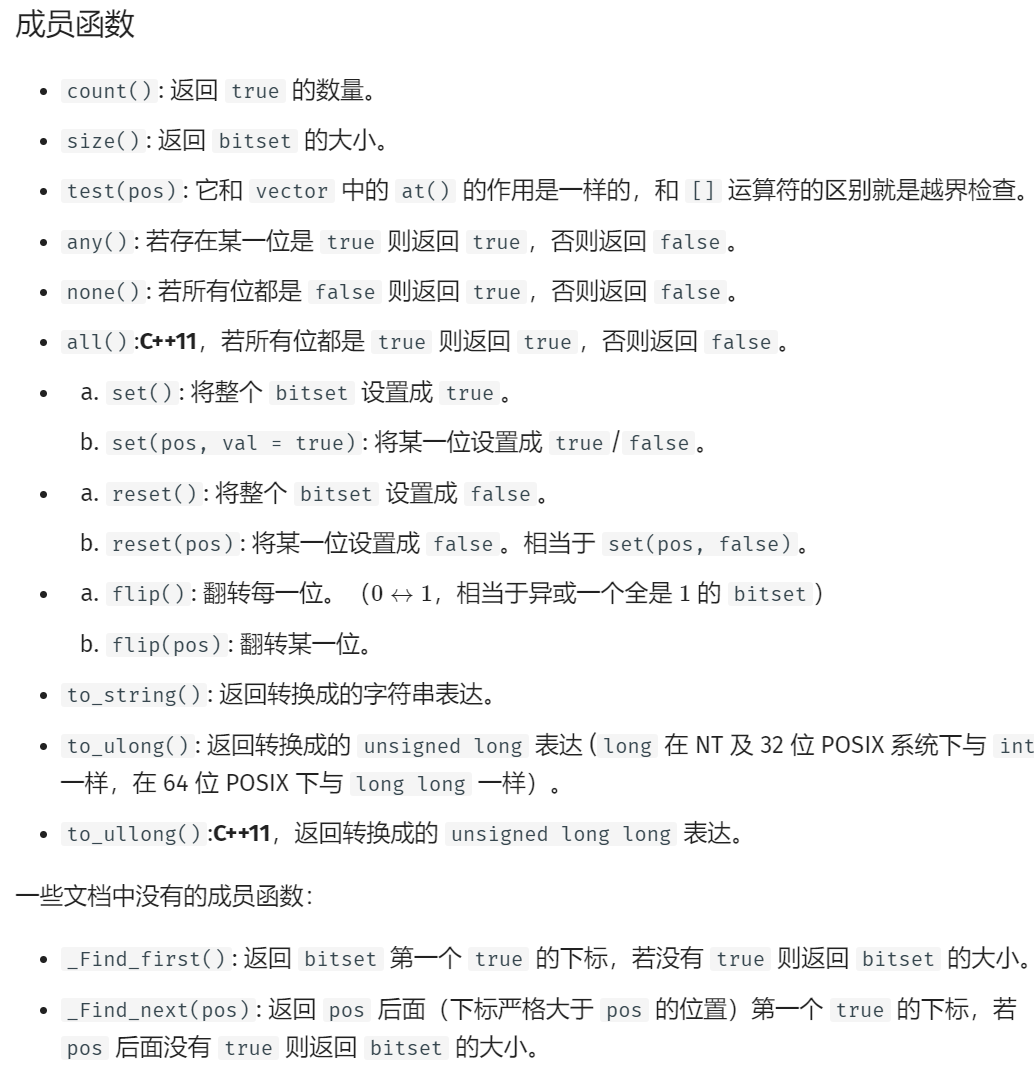
\includegraphics[width=10cm]{images/bitset.png}
\end{figure}